\subsection{Search tree}
In order to find the best possible move starting from a position, algorithms build search trees. 
Exemple with Tic-Tac-Toe: \cite{images_annexes}
\begin{figure}[H]
	\centering
	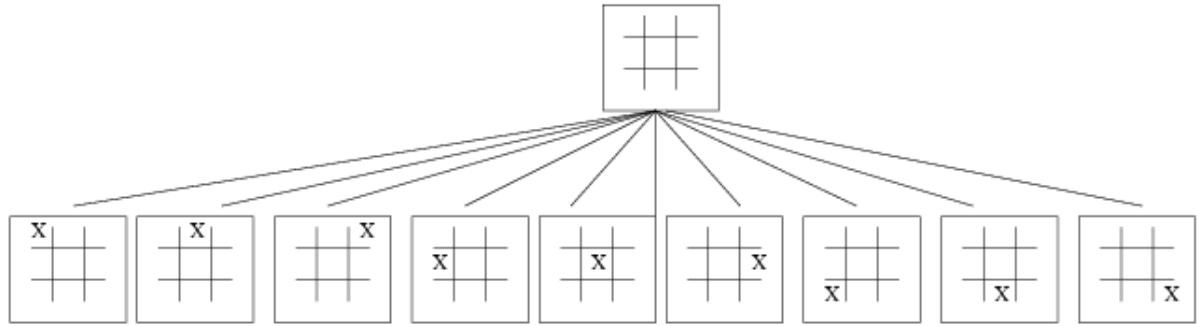
\includegraphics[width=15cm]{5_Annexes/img/Tree1.png}
	\caption{\label{fig:tree1}All possible moves starting from an empty board.}
\end{figure}
\noindent
\begin{figure}[H]
	\centering
	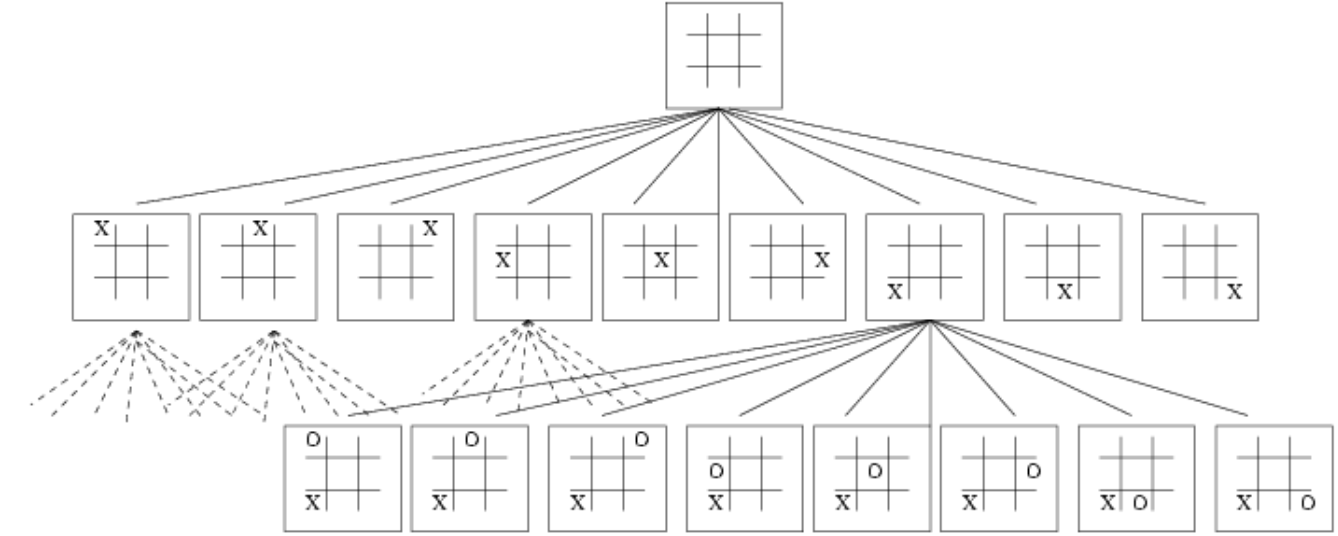
\includegraphics[width=15cm]{5_Annexes/img/Tree2.png}
	\caption{\label{fig:tree2}List of all possible moves for the other player.}
\end{figure}
\noindent
Continue this expansion until a winning position for the required player is found. Such tree is called a search tree.
\bigskip\\
However depending of the number of moves possible for the chosen game, the tree might be too large to be explored completely. Therefore in order to simplify the searches, the algorithm will try to evaluate the odds of winning in each position explored. Such value will be stored in each node and used by the program in order to find the best move to play given a position.